\documentclass[11pt,a4paper]{article}
\usepackage[margin=2.2cm]{geometry}
\usepackage[T1]{fontenc}
\usepackage{lmodern}
\usepackage{amsmath,amssymb}
\usepackage{booktabs,tabularx,multirow}
\usepackage{graphicx}
\usepackage{xcolor}
\usepackage{tikz}
\usetikzlibrary{positioning,arrows.meta,fit}
\usepackage[hidelinks]{hyperref}
\usepackage{enumitem}
\setlist{nosep,leftmargin=*}

\graphicspath{{../trained_model5TeV/}}
\newcommand{\nutau}{\ensuremath{\nu_\tau}}
\newcommand{\nue}{\ensuremath{\nu_e}}
\newcommand{\code}[1]{\texttt{#1}}
\newcolumntype{Y}{>{\raggedright\arraybackslash}X}

\title{GAT-based $\nu_\tau$ / $\nu_e$ classifier for 5\,TeV cascades\\[2pt]
\large Data, inputs, network architectures, training and results to date}
\author{Analysis code: \code{doublepulse/gnn/Analysis}}
\date{20 October 2026}

\begin{document}
\sloppy
\maketitle
\tableofcontents

%======================================================================
\section{Goal and overview}
The classifier separates \nutau\ charged-current events (signal, \code{pid}\,=\,16) from \nue\ events
(background, \code{pid}\,=\,11) in the 5\,TeV IceCube Virgo simulation. At these energies the tau decay length is
$\gamma c\tau \approx (5\,\mathrm{TeV}/1.777\,\mathrm{GeV})\times 87\,\mu\mathrm{m}\approx 25$\,cm (less for the
visible tau energy), i.e.\ $\sim$1\,ns of light travel, well below the $\sim$5--8\,ns pulse spacing of the unfolded
waveforms. A double pulse inside a single DOM is therefore not resolvable; the working hypothesis is that the
\nutau\ topology leaves a subtle imprint on the charge-versus-time pattern of the DOMs around the brightest DOM.

The network is a graph attention network (GAT) on a DOM-level graph with a per-DOM pulse encoder; no CNN is used.
(A CNN branch on a ``brightest-string image'' was tested and dropped, Sec.~\ref{sec:results}.) Everything is
implemented in \code{trainer.py}, \code{trainer\_domenc.py} and the driver \code{train.py}.

%======================================================================
\section{Simulation samples}
\subsection{Sources}
\begin{itemize}
  \item Directory \code{/mnt/ufs18/rs/IceCube/lownutau/sqlite/virgo\_v4/}
  \item \nue: \code{nue\_5TeV\_train/}, files \code{nue\_5TeV\_0228\{55,56,57\}.db}
  \item \nutau: \code{nutau\_5TeV\_train/}, files \code{nutau\_5TeV\_0228\{58,59,60\}.db}
  \item Tables used: \code{CleanedROIPulses} (per pulse: \code{dom\_x, dom\_y, dom\_z, dom\_time, charge}),
        \code{truth}, \code{reco}. Note: \code{reco.brightest\_om\_brightest\_string\_id} is the brightest DOM's
        \emph{number on its string} (1--60), not a string id ($\approx$82\% agreement with our own brightest DOM; the
        reco uses all pulses, we apply a 0.1\,PE threshold).
\end{itemize}

\subsection{Event selection when combining (\code{virgo/merge-5TeV-moresamples.py})}
\begin{itemize}
  \item \code{reco.brightest\_om\_brightest\_string\_PE} $>$ 10 and \code{truth.seed\_string} not null.
  \item Eligible pool: 162\,214 \nutau\ and 238\,192 \nue\ events.
  \item \code{event\_no} is offset by $10^6\times$(file index) so events are unique in the combined DB.
\end{itemize}

\subsection{Samples produced}
\begin{tabularx}{\textwidth}{lYl}
\toprule
File (\code{Analysis/data/}) & Content & Use\\
\midrule
\code{combined\_\{nutau,nue\}\_5TeV.db} & all eligible events & full training (earlier runs)\\
\code{\dots\_1k.db} & 1\,000 random events / flavour (seed 42) & smoke tests\\
\code{\dots\_20k.db} & 20\,000 random / flavour & first comparisons\\
\code{\dots\_40k.db} & 40\,000 random / flavour & current training\\
\code{\dots\_40k\_matched.db} & 40\,000 / flavour, matched in true (cos\,zenith, $\log_{10}E$), $20\times20$ bins & not used (see Sec.~\ref{sec:confound})\\
\bottomrule
\end{tabularx}

\medskip
Sampling (\code{--n-events N}) draws uniformly from the eligible pool, so the dataset composition matches the full
sample; the 1k sample is a subset of the 20k sample. The extraction reads only the selected rows (temporary-table
join), never whole pulse tables.

\subsection{Kinematic difference between the samples}\label{sec:confound}
The \nutau\ and \nue\ sets have different true direction and energy distributions (median
$\cos\theta_\mathrm{zen}$ 0.54 vs.\ 0.09; median $\log_{10}E/\mathrm{GeV}$ 4.31 vs.\ 4.19). A gradient-boosted tree on
\emph{true} $(\cos\theta,\log_{10}E)$ alone reaches AUC $=0.694$ on the random 20k samples, and $0.534$ after matching
(0.509 with $20\times20$ matching bins). Direction-dependent quantities (e.g.\ arrival times of DOMs above/below the
brightest DOM) therefore carry a sample-level, not flavour-level, signal. Reconstructed direction + energy give AUC
$\approx0.60$ even after matching, mostly because \nutau\ events reconstruct dimmer at the same true energy (energy
carried away by neutrinos) --- that part is genuine physics. Current policy: no event selection on truth; results are
also reported as AUC \emph{within} bins of true $\cos\theta$ and $\log_{10}E$ (Sec.~\ref{sec:eval}).

%======================================================================
\section{Event preprocessing}
Implemented in \code{trainer.preprocess\_event\_hits}; identical for all networks.
\begin{enumerate}
  \item Keep pulses within 1500\,ns of the event's first pulse; times are relative to that pulse.
  \item Keep pulses with charge $>$ \code{--charge\_threshold} (0.1\,PE).
  \item Map each pulse to a string with a KD-tree on the geometry (\code{geometry\_clean.csv}, 86 strings $\times$ 60 DOMs);
        drop pulses more than 50\,m from any DOM.
  \item \textbf{Optional per-DOM charge cut} (\code{--min\_dom\_charge}, used at 10\,PE in the current runs): sum the
        charge per DOM (string, $z$) and remove every DOM below the threshold, with all its pulses.
  \item Validity: $\geq4$ pulses on $\geq2$ strings, otherwise the event is dropped.
  \item Classes are balanced 1:1 by randomly subsampling the larger class (seed 42); the train/validation split
        (85/15) is stratified by flavour.
\end{enumerate}

\paragraph{Effect of the 10\,PE DOM cut} (600 random events/flavour, \code{notebooks/dom-charge-cut.ipynb}):
DOMs per event drop from a median of 75 to 15 (77\% of DOMs removed) while only 26\% of pulses and 12\% of the
charge are removed. 83\% of events still pass the validity cut (83.7\% \nutau, 83.0\% \nue); the loss is concentrated
at low energy ($\sim$55--65\% survival at $\log_{10}E\approx3$). The k-NN graph becomes less string-local: events whose
brightest DOM has no edge to another string drop from 36\% to 5\%. On the 40k samples: 33\,077 \nutau\ and 33\,712
\nue\ events survive, balanced to 33\,077 each.

%======================================================================
\section{Input representation}
\subsection{DOM graph (\code{trainer.event\_to\_dom\_graph})}
One node per hit DOM; pulses on the same DOM are aggregated. Normalisations: $s_{xyz}=500$\,m, $s_t=500$\,ns.

\begin{tabularx}{\textwidth}{rlY}
\toprule
\# & Node feature & Definition\\
\midrule
0--2 & \code{x\_norm, y\_norm, z\_norm} & DOM position / $s_{xyz}$\\
3 & \code{q\_log} & $\ln(1+Q_\mathrm{DOM})$\\
4 & \code{q\_frac} & $Q_\mathrm{DOM}/Q_\mathrm{event}$\\
5 & \code{t\_first} & first pulse time / $s_t$\\
6 & \code{t\_mean} & charge-weighted mean time / $s_t$\\
7 & \code{t\_spread} & std of pulse times / $s_t$\\
8 & \code{n\_pulses} & number of pulses / 10\\
9 & \code{dom\_depth\_rank} & rank of the DOM's depth among hit DOMs of its string, in $[0,1]$\\
10 & \code{z\_rel} & $(z-\bar z_Q)/s_{xyz}$, $\bar z_Q$ = charge-weighted event depth\\
11 & \code{distance\_to\_cascade} & distance to the reconstructed cascade vertex (normalised units)\\
12 & \code{log\_energy} & $\log_{10}\max(E_\mathrm{reco}/\mathrm{TeV},0.05)/6$\\
\bottomrule
\end{tabularx}

\medskip
\textbf{Edges}: $k$-nearest neighbours in 3D ($k=8$, no self loops). Without the DOM cut, 83\% of edges connect DOMs on
the same string. \textbf{Edge features} (6, used by \code{trainer} and \code{trainer\_domenc}):
$\Delta x,\Delta y,\Delta z$ and distance (normalised), $\Delta t_\mathrm{first}$ (normalised), same-string flag.

\subsection{Per-pulse features (\code{trainer\_domenc.dom\_pulse\_features})}
Every DOM keeps its full, time-ordered pulse list (median 3 pulses per DOM, 99th percentile 68, max $\sim$140;
brightest DOM median $\sim$52 pulses at $\sim$8\,ns spacing). Per pulse:
$\Delta t_\mathrm{first}/s_t$; $\ln(1+\Delta t_\mathrm{prev}/\mathrm{ns})/\ln(1+500)$; $\ln(1+q)$; $q/Q_\mathrm{DOM}$;
cumulative charge fraction on the DOM. Stored as \code{pulse\_x} with a pulse$\to$DOM index \code{pulse\_dom}
(shifted correctly when graphs are batched).

\subsection{Brightest-string image (diagnostic only, not a network input)}
\code{trainer\_domenc.brightest\_string\_image} builds a fixed-size view of the brightest-DOM neighbourhood, used for
event displays and feature studies. It was the input of the dropped CNN branch; the GAT does not use it.
Image size $2\times7\times220$:
\begin{itemize}
  \item channel 0: the brightest DOM $\pm3$ DOMs on its string (by DOM number, so unhit DOMs are empty rows);
  \item channel 1: the other string with the largest charge within $\pm56$\,m of the brightest DOM's depth, centred on
        its DOM closest to that depth (in $\sim$40\% of events this string sees $>30\%$ of the brightest string's charge
        at that depth; median distance 125\,m);
  \item time axis: 5\,ns bins from $-100$ to $+1000$\,ns relative to the brightest DOM's first pulse (98\% of the
        brightest-string charge falls inside);
  \item value: $\log_{10}(1+10^3\,q/Q_b)/3$, $q$ = charge in the bin, $Q_b$ = brightest-DOM charge;
  \item 4 scalars: string-2 distance/125\,m, string-2/string-1 charge ratio at that depth, string-2 depth offset/17\,m,
        string-2 present.
\end{itemize}
Event displays: \code{notebooks/brightest-string-image.ipynb}.\\
Prototype study: \code{notebooks/brightest-features-abc.ipynb}.

\subsection{Event-level PCA features (no longer used)}
13 features: spatial PCA variances (\code{pc1/2/3\_var}, \code{elongation}, \code{pc1\_pc2\_sum}), loadings of the
first PC of standardised $(t,q,z)$ (\code{depth/time/charge\_loading}), counts (\code{n\_strings}, \code{n\_doms},
\code{n\_hits}), \code{total\_charge}, \code{log\_energy}. After kinematic matching the 9 shape features have
AUC 0.47--0.53; only the brightness-related ones separate (AUC $\approx$0.42--0.44). The PCA branch is disabled
(\code{--no\_pca}) in all current runs.

\subsection{Auxiliary truth targets (optional, not used now)}
\code{--aux\_weight}\,$>0$ adds a regression head predicting standardised true $\log_{10}E$ and the true direction unit
vector; loss = BCE + \code{aux\_weight}\,$\times$\,MSE. Truth is only a target, never an input.

%======================================================================
\section{Network architectures}
All networks output one logit; $\sigma(\text{logit})$ is the \nutau\ score. Hidden width $h=64$, 4 attention heads
(concatenated, so 256 features after each graph layer).

\begin{table}[h]
\centering\small
\begin{tabularx}{\textwidth}{lYr}
\toprule
Network (\code{--trainer}) & Layers & Parameters\\
\midrule
\code{trainer\_noedge} & node MLP $13\to64$ $\to$ $3\times$GATConv (no edge features) $\to$ sum-pool $\oplus$ mean \code{q\_log} $\to$ (+PCA MLP) $\to$ MLP $\to$ logit & 171\,457 (with PCA)\\
\code{trainer} & node MLP $\to$ TransformerConv (edge features) $\to$ $2\times$GATConv (no edge features) $\to$ same readout & 219\,841 (no PCA)\\
\code{trainer\_domenc} & pulse encoder $\to$ node MLP $\to$ $3\times$GATv2Conv (edge features) $\to$ same readout & 336\,418 (no PCA)\\
\code{trainer\_domenc} + readout/residual & as above, multi readout and residual GAT layers (Sec.~\ref{sec:gatopts}) & 418\,595\\
\code{trainer\_domenc} + all options & + brightest-relative node features, fine-time/causality edge features (k-NN or fully connected graph) & 420\,451\\
\bottomrule
\end{tabularx}
\caption{Network variants (all without CNN). Each graph layer: GAT$\to$BatchNorm$\to$ReLU$\to$Dropout(0.4). Default
readout: global sum pool (257 = 256 + mean \code{q\_log}). Final MLP: Linear$\to$64$\to$ReLU$\to$Dropout(0.3)$\to$Linear$\to$1.}
\end{table}

\subsection{GAT with per-DOM pulse encoder (\code{trainer\_domenc})}
\begin{center}
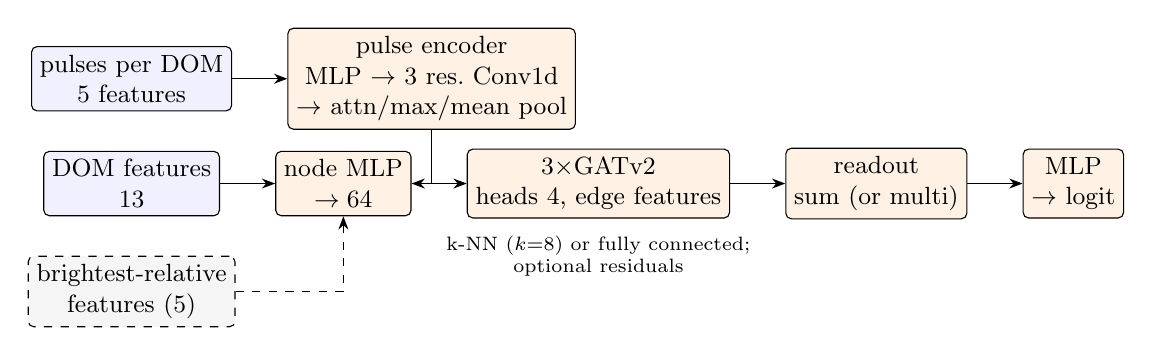
\begin{tikzpicture}[node distance=5mm and 7mm, >=Stealth,
  box/.style={draw, rounded corners=2pt, align=center, font=\small, minimum height=8mm, inner sep=3pt},
  dat/.style={box, fill=blue!6}, net/.style={box, fill=orange!10}, opt/.style={box, dashed, fill=gray!8}]
\node[dat] (pul) {pulses per DOM\\$5$ features};
\node[net, right=of pul] (penc) {pulse encoder\\MLP $\to$ 3 res.\ Conv1d\\$\to$ attn/max/mean pool};
\node[dat, below=of pul] (nod) {DOM features\\13};
\node[opt, below=of nod] (bf) {brightest-relative\\features (5)};
\node[net, right=of nod] (nmlp) {node MLP\\$\to64$};
\node[net, right=of nmlp] (gat) {$3\times$GATv2\\heads 4, edge features};
\node[net, right=of gat] (pool) {readout\\sum (or multi)};
\node[net, right=of pool] (fus) {MLP\\$\to$ logit};
\draw[->] (pul) -- (penc); \draw[->] (penc) |- (nmlp); \draw[->] (nod) -- (nmlp); \draw[->, dashed] (bf) -| (nmlp);
\draw[->] (nmlp) -- (gat); \draw[->] (gat) -- (pool); \draw[->] (pool) -- (fus);
\node[font=\scriptsize, below=1mm of gat, align=center] {k-NN ($k{=}8$) or fully connected;\\optional residuals};
\end{tikzpicture}
\end{center}
Dashed: optional (Sec.~\ref{sec:gatopts}).

\paragraph{Pulse encoder} Per-pulse Linear $5\to32$ + ReLU; three residual 1D convolutions along each DOM's
time-ordered pulse sequence (kernel 3, dilations 1, 2, 4; receptive field 15 pulses), with padding re-zeroed after each
layer; pooling over the DOM's pulses by learned attention, max and mean; Linear $96\to32$ + ReLU (12\,641 parameters).

\paragraph{Graph layers} $3\times$\code{GATv2Conv}($\cdot$, 64, heads 4, \code{edge\_dim}=6): attention depends on both
endpoints and on the edge features (unlike GATConv~v1, whose neighbour ranking is the same for every query node).
302\,592 parameters.

\subsection{GAT-branch options}\label{sec:gatopts}
Switched on from \code{train.py}; all are computed inside the model from the cached node features, so they need no
dataset rebuild. With all options off the network is exactly the one above.
\begin{tabularx}{\textwidth}{lY}
\toprule
\code{--gat\_readout multi} & event embedding = sum $\oplus$ mean $\oplus$ max $\oplus$ attention pooling $\oplus$ the brightest DOM's
  final embedding $\oplus$ mean \code{q\_log} (1281-d), so the brightest-neighbourhood signal is not diluted by the sum\\
\code{--gat\_residual} & residual connections around the three GATv2 layers (linear projection for the first)\\
\code{--bright\_feats} & 5 node features relative to the event's brightest DOM: distance/125\,m, $\mathrm{asinh}(\Delta t_\mathrm{first}/50\,\mathrm{ns})$,
  same-string flag, depth offset along that string/17\,m, $\Delta$\code{q\_log}\\
\code{--extra\_edges} & 2 edge features at fine time scale: $\mathrm{asinh}(\Delta t/20\,\mathrm{ns})$ and the causality residual
  $\mathrm{asinh}((|\Delta t|-d/c_\mathrm{ice})/20\,\mathrm{ns})$, $c_\mathrm{ice}=0.221$\,m/ns\\
\code{--full\_graph} & every DOM attends to every DOM of its event instead of its 8 nearest neighbours (cheap after the
  10\,PE cut: $\sim$15 DOMs/event); edge features computed for all pairs\\
\bottomrule
\end{tabularx}

\paragraph{Dropped: CNN branch} A 2D CNN on the brightest-string image (3 conv layers, 139k parameters), fused with the
GAT readout before the final MLP, was trained once (Sec.~\ref{sec:results}). It peaked early and overfitted, and the
image shows almost no flavour difference, so it is not used. The code remains in \code{trainer\_domenc.py}
(\code{BrightestStringCNN}, \code{--use\_image}), off by default.

%======================================================================
\section{Training}
\begin{tabularx}{\textwidth}{lY}
\toprule
Loss & \code{BCEWithLogitsLoss}, \code{pos\_weight}$=n_\mathrm{neg}/n_\mathrm{pos}$ (=1 after balancing)\\
Optimiser & AdamW, lr $3\times10^{-4}$, weight decay $5\times10^{-4}$, gradient clipping 1.0, batch 64\\
LR schedule & \code{ReduceLROnPlateau} on validation BCE: $\times0.5$ after 5 epochs without improvement, min $10^{-6}$
               (default; \code{--lr\_scheduler exp} gives the earlier $\times0.98$/epoch)\\
Early stopping & on validation AUC, patience 25 (job scripts), max 150 epochs; the best-AUC weights are saved\\
Data cache & built dataset saved under \code{dataset\_cache\_5TeV/}, keyed by DB list, cuts and graph version;
             \code{--build\_only} builds it in a separate job before parallel trainings\\
Reproducibility & seed 42 (sampling, balancing, split, torch)\\
Outputs & \code{hybrid\_weights.pt}, \code{eval\_val.npz} (validation scores, truth targets, history incl.\ LR),
          \code{run\_config.json}, training curves\\
\bottomrule
\end{tabularx}

\medskip
Typical cost on an A100: dataset build $\sim$23\,min (40k/flavour with the 10\,PE cut); \code{trainer\_domenc}
$\sim$30--40\,s per epoch; 40--65 epochs to early stopping. Jobs: \code{job-scripts/submit\_test40k\_cut10.sh} (cache +
GAT reference) and \code{submit\_test40k\_gat\_ablation.sh} (GAT options), 3.5\,h limit.

%======================================================================
\section{Evaluation}\label{sec:eval}
\code{plot\_eval.py} produces, per run: training history, ROC with bootstrap 95\% CI on the AUC, score distributions,
and (with an aux head) energy/direction regression plots; across runs: ROC comparison, AUC in bins of true
$\cos\theta$ and true $\log_{10}E$, and \code{summary.csv}. The \textbf{AUC within true-direction bins} is the closest
measure of flavour separation alone, because the direction difference between the samples cannot help inside a bin.
Live monitoring: \code{inspect-training-live.ipynb}.

%======================================================================
\section{Results to date}\label{sec:results}
\begin{table}[h]
\centering\small
\begin{tabularx}{\textwidth}{lYccc}
\toprule
Sample & Network & Val.\ AUC & AUC in $\cos\theta$ bins & best ep.\\
\midrule
Full (Virgo-Run1, earlier) & summary GNN, LR halving & 0.661 & -- & 40\\
\midrule
\multirow{3}{*}{20k random} & \code{trainer} (PCA) & 0.652 & -- & 54\\
 & \code{trainer\_domenc} (PCA) & 0.644 & -- & 36\\
 & \code{trainer\_domenc} (no PCA; cancelled) & 0.650 (ep.\ 29) & -- & --\\
\midrule
\multirow{2}{*}{40k random} & \code{trainer}, no PCA, aux 0.5 & 0.659 [0.649, 0.668] & 0.553 & 36\\
 & \code{trainer\_domenc}, no PCA, aux 0.5 & 0.663 [0.653, 0.672] & 0.558 & 39\\
\midrule
\multirow{5}{*}{\shortstack[l]{40k random,\\DOM $\geq$ 10\,PE}} & \code{trainer\_domenc} (GAT reference) & 0.656 [0.645, 0.668] & 0.556 & 24\\
 & GAT + CNN image branch (dropped; cancelled ep.\ 25) & 0.643 & -- & 10\\
 & GAT + multi readout + residual & \multicolumn{3}{c}{running}\\
 & \dots\ + brightest/causality features & \multicolumn{3}{c}{running}\\
 & \dots\ + fully connected graph & \multicolumn{3}{c}{running}\\
\bottomrule
\end{tabularx}
\caption{Validation results. Square brackets: bootstrap 95\% CI. The 40k aux runs predicted energy with
$\sigma(\log_{10}E)=0.44$ and direction with a median error of 55$^\circ$. With the 10\,PE cut the validation set
has 9\,924 events; the GAT reference reaches 0.668 averaged over true-energy bins.}
\end{table}

\paragraph{CNN branch (dropped)} With the 10\,PE cut, GAT + CNN peaked at AUC 0.643 after 10 epochs, below the GAT
alone (0.656), and then overfitted (training loss 0.61 vs.\ validation 0.70 at epoch 25). This agrees with the feature
study below: the image carries almost no flavour information beyond what the GAT already sees.

\begin{figure}[h]
\centering
\includegraphics[width=0.42\textwidth]{test40k_comparison/roc_comparison.png}\hfill
\includegraphics[width=0.56\textwidth]{test40k_comparison/auc_vs_truth.png}
\caption{40k random samples, no PCA, aux 0.5. Left: ROC (\code{trainer} vs.\ \code{trainer\_domenc}). Right: AUC within
bins of true $\cos\theta$ (left) and true $\log_{10}E$ (right). Inside direction bins the AUC drops to $\approx0.55$,
i.e.\ roughly two thirds of the separation above 0.5 comes from the direction difference between the samples.}
\end{figure}

\paragraph{Feature studies} (kinematically matched, 4\,178 events/flavour, gradient-boosted trees, 5-fold CV;
\code{notebooks/brightest-features-abc.ipynb}): event-level brightness features 0.566; brightest-string image 0.553;
brightest-relative neighbour timing/charge and causality residuals 0.532; all combined 0.564. The mean
brightest-string images of the two flavours are almost identical (12 of 1540 pixels with $|z|>3$, $\approx$4 expected
from noise).

%======================================================================
\section{Open points}
\begin{itemize}
  \item The flavour-only separation (within-direction-bin AUC $\approx0.55$) is far below the headline AUC; decide whether
        to remove the direction difference by per-event loss weights (no events dropped) or keep reporting both numbers.
  \item The 10\,PE DOM cut does not reduce performance (0.656 vs.\ 0.663 without it, the latter with auxiliary
        targets) while cutting the graph size $\sim$5$\times$. The running ablation tests the GAT-branch options
        (Sec.~\ref{sec:gatopts}).
  \item The 17\% of events lost to the DOM cut are mostly single-string and low-energy; the validity cut could be relaxed
        to $\geq2$ DOMs if they are wanted back.
\end{itemize}

%======================================================================
\section{File map}
\begin{tabularx}{\textwidth}{lY}
\toprule
\code{virgo/merge-5TeV-moresamples.py} & builds combined / sampled / matched DBs\\
\code{trainer.py} & preprocessing, DOM graph, dataset class, \code{trainer} network\\
\code{trainer\_domenc.py} & pulse encoder, GATv2 network and its options; brightest-string image (diagnostic);
  unused CNN branch\\
\code{trainer\_noedge.py} & original GAT without edge features\\
\code{train.py} & training driver (\code{--trainer}, \code{--no\_pca}, \code{--min\_dom\_charge}, \code{--gat\_readout},
  \code{--gat\_residual}, \code{--bright\_feats}, \code{--extra\_edges}, \code{--full\_graph}, \dots)\\
\code{plot\_eval.py} & evaluation plots and \code{summary.csv}\\
\code{job-scripts/} & SLURM jobs (\code{job\_test40k.sh}, \code{submit\_test40k\_cut10.sh}, \dots)\\
\code{notebooks/} & feature studies and displays\\
\code{backup/} & copies of every script before modification\\
\bottomrule
\end{tabularx}

\end{document}
